\documentclass[tikz, border=2mm]{standalone}
\usetikzlibrary{positioning, arrows.meta, shapes.geometric, calc}

\begin{document}

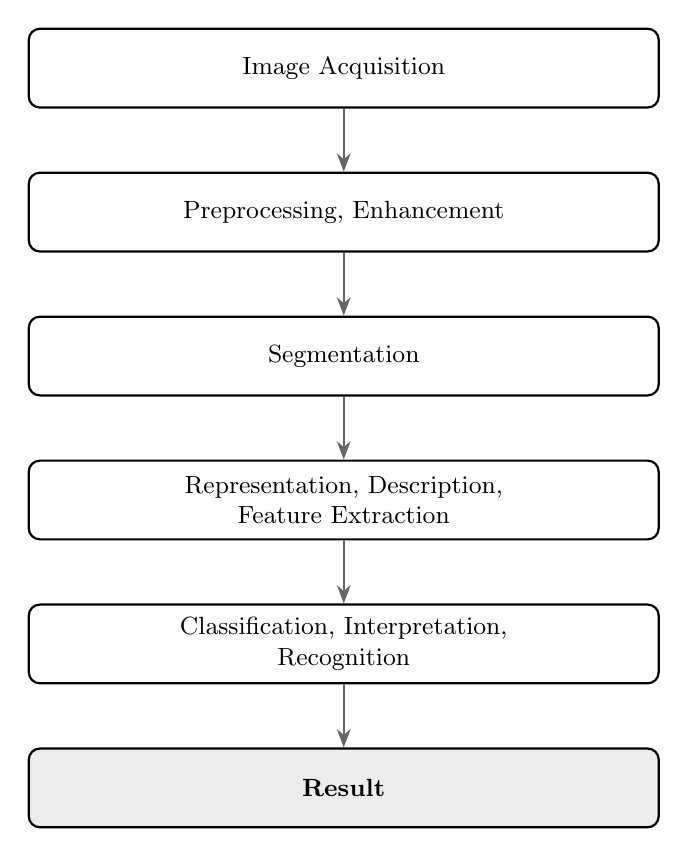
\begin{tikzpicture}[
    node distance=0.8cm,
    every node/.style={
        draw,
        rounded corners,
        align=center,
        minimum width=8cm,
        minimum height=1cm,
        font=\small,
        fill=white,
        thick
    },
    arrow/.style={-Stealth, thick, color=gray!80!black}
]

    \node (a) {Image Acquisition};
    \node (b) [below=of a] {Preprocessing, Enhancement};
    \node (c) [below=of b] {Segmentation};
    \node (d) [below=of c] {Representation, Description, \\ Feature Extraction};
    \node (e) [below=of d] {Classification, Interpretation, \\ Recognition};
    \node (f) [below=of e, fill=gray!15] {\textbf{Result}};

    \draw[arrow] (a) -- (b);
    \draw[arrow] (b) -- (c);
    \draw[arrow] (c) -- (d);
    \draw[arrow] (d) -- (e);
    \draw[arrow] (e) -- (f);

\end{tikzpicture}

\end{document}